%!TEX root = mieic.tex
\chapter{Conclusões e Trabalho Futuro} \label{chap:concl}

\section*{}

\section{Perspetiva de Solução}

A solução pensada para alcançar todos os objetivos propostos passa pela criação de uma framework, que facilite o desenvolvimento de aplicações para ecrãs públicos usando para esse efeito diferentes tecnologias. É possível distinguir entre o servidor e a parte que diz respeito ao cliente, usando para o servidor, Java e para o cliente HTML, CSS e Javascript.
Após o desenvolvimento da framework serão criados pequenos exemplos de aplicações que serão sujeitos a testes reais em ecrãs públicos.

\section{Plano de Trabalho}

De forma a alcançar os objetivos propostos, estruturei o desenvolvimento do trabalho da seguinte forma, como é possível ver na figura~\ref{fig:plano}:

\begin{figure}[h]
\centering
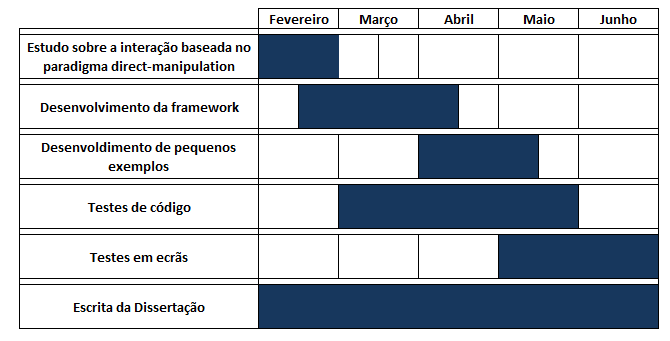
\includegraphics[width=\columnwidth]{plano.png}
\caption {Plano de trabalho}
\label{fig:plano}
\end{figure}

No mês de fevereiro realizarei de forma pormenorizada o estudo sobre o paradigma \textit{direct-manipulation}, de forma a perceber e escolher a melhor forma de como desenvolver ou integrar num toolkit uma arquitetura que facilite o desenvolvimento de aplicações para ecrãs públicos. Ainda durante esta fase, darei início ao desenvolvimento, acompanhado dos respetivos testes de código. A partir de abril, após a fase anterior estar praticamente concluída poderei desenvolver pequenos exemplos para demonstrar o trabalho realizado, aos quais serão realizados alguns testes reais em ecrãs existentes.
A dissertação será escrita ao longo de todo o desenvolvimento, terminando o projeto no final do mês junho. 